%description: Book template

% template of document for LaTeX
% (C) Xavier Perseguers 2002 - xavier.perseguers@epfl.ch

\documentclass[a4paper,11pt]{book}
%\documentclass[a4paper,11pt,makeidx]{book} <== may need this to generate index

%  makeindex NEMO_BDY_tools     <== to regenerate the index
%  bibtex         NEMO_BDY_tools	<== to generate  the bibliography

% ================================================================
% HEADERS DEFINITION
% ================================================================

\usepackage[french]{babel}
%\usepackage{color}
\usepackage{xcolor}
%\usepackage{graphics}				% allows insertion of pictures
\usepackage{graphicx}				% allows insertion of pictures
\usepackage[capbesideposition={top,center}]{floatrow} % allows captions
\floatsetup[table]{style=plaintop}                                   % beside pictures
\usepackage[margin=10pt,font={small},labelsep=colon,labelfont={bf}]{caption} % Gives small font for captions
\usepackage{enumitem}                          % allows non-bold description items
%\usepackage{colortbl}                           % gives coloured panels behind table columns

%hyperref
\usepackage[					%
  pdftitle={NEMO BDY tools},	%
  pdfauthor={James Harle},		% pdfsubject={The preprint document class
                           				% elsart},% pdfkeywords={diapycnal diffusion,numerical mixing,z-level models},%
  pdfstartview=FitH,				%
  bookmarks=true,				%
  bookmarksopen=true,			%
  breaklinks=true,				%
  colorlinks=true,				%
  linkcolor=blue,anchorcolor=blue,	%
  citecolor=blue,filecolor=blue,		%
 menucolor=blue,                   	%
  urlcolor=blue]{hyperref}
%  usage of exteranl hyperlink :  \href{mailto:my_address@wikibooks.org}{my\_address@wikibooks.org}
%                                                 \url{http://www.wikibooks.org}
%                                     or         \href{http://www.wikibooks.org}{wikibooks home}



%%%% page styles etc................
\usepackage{fancyhdr}
\pagestyle{fancy}
% with this we ensure that the chapter and section
% headings are in lowercase.
\renewcommand{\chaptermark}[1]{\markboth{#1}{}}
\renewcommand{\sectionmark}[1]{\markright{\thesection.\ #1}}
\fancyhf{}             % delete current setting for header and footer
\fancyhead[LE,RO]{\bfseries\thepage}
\fancyhead[LO]{\bfseries\hspace{-0em}\rightmark}
\fancyhead[RE]{\bfseries\leftmark}
\renewcommand{\headrulewidth}{0.5pt}
\renewcommand{\footrulewidth}{0pt}
\addtolength{\headheight}{2.6pt}   % make space for the rule
%\addtolength{\headheight}{1.6pt}   % make space for the rule
\fancypagestyle{plain}{
  \fancyhead{}         % get rid of headers on plain pages
  \renewcommand{\headrulewidth}{0pt}  % and the line
}


%%%%  Section number in Margin.......
% typeset the number of each section in the left margin, with the start of each instance of
% sectional heading text aligned with the left hand edge of  the body text.
\makeatletter
\def\@seccntformat#1{\protect\makebox[0pt][r]{\csname the#1\endcsname\quad}}
\makeatother

% Leave blank pages completely empty, w/o header
\makeatletter
\def\cleardoublepage{\clearpage\if@twoside \ifodd\c@page\else
  \hbox{}
  \vspace*{\fill}
  \vspace{\fill}
  \thispagestyle{empty}
  \newpage
  \if@twocolumn\hbox{}\newpage\fi\fi\fi}
\makeatother

%%%% define the chapter  style ................
\usepackage{minitoc}				%In French : \usepackage[french]{minitoc}
%\usepackage{mtcoff}				% invalidate the use of minitocs
\usepackage{fancybox}

\makeatletter
\def\LigneVerticale{\vrule height 5cm depth 2cm\hspace{0.1cm}\relax}
\def\LignesVerticales{%
  \let\LV\LigneVerticale\LV\LV\LV\LV\LV\LV\LV\LV\LV\LV}
\def\GrosCarreAvecUnChiffre#1{%
  \rlap{\vrule height 0.8cm width 1cm depth 0.2cm}%
 \rlap{\hbox to 1cm{\hss\mbox{\color{white} #1}\hss}}%
  \vrule height 0pt width 1cm depth 0pt}
\def\GrosCarreAvecTroisChiffre#1{%
  \rlap{\vrule height 0.8cm width 1.6cm depth 0.2cm}%
 \rlap{\hbox to 1.5cm{\hss\mbox{\color{white} #1}\hss}}%
  \vrule height 0pt width 1cm depth 0pt}

\def\@makechapterhead#1{\hbox{%
   \huge
    \LignesVerticales
    \hspace{-0.5cm}%
    \GrosCarreAvecUnChiffre{\thechapter}
    \hspace{0.2cm}\hbox{#1}%
%    \GrosCarreAvecTroisChiffre{\thechapter}
%    \hspace{1cm}\hbox{#1}%
%}\par\vskip 2cm}
}\par\vskip 1cm}
\def\@makeschapterhead#1{\hbox{%
   \huge
    \LignesVerticales
    %\hspace{0.5cm}%
    \hbox{#1}%
}\par\vskip 2cm}
\makeatother

%\def\thechapter{\Roman{chapter}}   	% chapter number to be Roman


%%%%           Mathematics...............
%\documentclass{amsart}
\usepackage{xspace}                              % helpd ensure correct spacing after macros
\usepackage{latexsym}
\usepackage{amssymb}
\usepackage{amsmath}
\allowdisplaybreaks[1]				% allow page breaks in the middle of equations
\usepackage{./TexFiles/math_abbrev}    % use maths shortcuts


\usepackage{times}				 	 % use times font for text
%\usepackage{mathtime}                          % font for illustrator to work (belleek fonts )
%\usepackage[latin1]{inputenc}                % allows some unicode removed (agn)


%%% essai commande
\newcommand{\nl} [1] {\texttt{\small {\textcolor{blue}{#1}} } }
\newcommand{\nlv} [1] {\texttt{\footnotesize#1}\xspace}
\newcommand{\smnlv} [1] {\texttt{\scriptsize#1}\xspace}

%%%% namelist & code display................................
\usepackage{alltt}  		%%  alltt for namelist
\usepackage{verbatim}  	%%  alltt for namelist
% namelists
\newcommand{\namdisplay} [1] {
\begin{alltt}

{\tiny \verbatiminput{#1}}
\end{alltt}
  \vspace{-10pt}
}
% code display
%\newcommand{\codedisplay} [1] { \begin{alltt} {\tiny  {\begin{verbatim} {#1}} \end{verbatim} }  \end{alltt}   }



%%%% commands for working with text................................
% command to "comment out" portions of text ({} argument) or not ({#1} argument)
\newcommand{\amtcomment}[1]{}   	% command to "commented out" portions of text or not (#1 in argument)
\newcommand{\sgacomment}[1]{}   	% command to "commented out" portions of
\newcommand{\gmcomment}[1]{}   	% command to "commented out" portions of
%                                    				% text that span line breaks
%Red (NR) or Yellow(WARN)
%\newcommand{\NR} {\colorbox{red}{#1}}
%\newcommand{\WARN} {{ \colorbox{yellow}{#1}} }



%%% index commands......................
\usepackage{makeidx}
%\usepackage{showidx}				% show the index entry

\newcommand{\mdl} [1] {\textit{#1.F90}\index{Modules!#1}}			%module (mdl)
\newcommand{\rou} [1] {\textit{#1}\index{Routines!#1}}				%module (routine)
\newcommand{\hf} [1] {\textit{#1.h90}\index{h90 file!#1}}				%module (h90 files)
\newcommand{\np} [1] {\textit{#1}\index{Namelist parameters!#1}}		%namelist parameter (nampar)
\newcommand{\jp} [1] {\textit{#1}\index{Model parameters!#1}}			%model parameter (jp)
\newcommand{\pp} [1] {\textit{#1}\index{Model parameters!#1}}		 	%namelist parameter (pp)
\newcommand{\ifile} [1] {\textit{#1.nc}\index{Input NetCDF files!#1.nc}}	%input NetCDF files (.nc)
\newcommand{\key} [1] {\textbf{key\_#1}\index{CPP keys!key\_#1}}	%key_cpp (key)
\newcommand{\NEMO} {\textit{NEMO}\xspace}						%NEMO (nemo)

%%%%   Bibliography   .............
\usepackage[nottoc, notlof, notlot]{tocbibind}
\usepackage[square, comma]{natbib}
\bibpunct{[}{]}{,}{a}{}{;}                           %suppress "," after "et al."
\providecommand{\bibfont}{\small}


% ================================================================
% FRONT PAGE
% ================================================================

%\usepackage{pstricks}
\title{
%\psset{unit=1.1in,linewidth=4pt} 	%parameters of the units for pstricks
% \rput(0,2){ 
\includegraphics[width=1.1\textwidth]{./TexFiles/Figures/logo_ALL.pdf}             } \\
% \vspace{0.1cm}
\vspace{-6.0cm}
%
\includegraphics[width=1.1\textwidth]{./TexFiles/Figures/logo_ALL.pdf}\\
\vspace{5.1cm}

\includegraphics[width=0.9\textwidth]{./TexFiles/Figures/NEMO_logo_Black.pdf} \\
\vspace{1.4cm}
\rule{345pt}{1.5pt} \\
\vspace{0.45cm}
{\Huge NEMO BDY Tools}
\rule{345pt}{1.5pt} \\
 }
%{ -- Draft --}   }
\date{\today \\
{\small  -- version 1.0 alpha --} \\
}
%\date{
%January 2012  \\
%{\small  -- version 3.4 --} \\
%~  \\
%\textit{\small Note du P\^ole de mod\'{e}lisation de l'Institut Pierre-Simon Laplace No 27 }\\
%\vspace{0.45cm}
%{ ISSN No 1288-1619.}
%}


\author{
\Large James Harle  \\
 \texttt{\small jdha@noc.ac.uk} \\
{\small National Oceanography Centre, Liverpool, UK}
}

\dominitoc
\makeindex  		%type this first :     makeindex -s NEMO.ist NEMO_book.idx

% ================================================================
%      Include ONLY order
% ================================================================

%\includeonly{./TexFiles/Chapters/Chap_MISC}
%\includeonly{./TexFiles/Chapters/Chap_ZDF}
%\includeonly{./TexFiles/Chapters/Chap_STP,./TexFiles/Chapters/Chap_SBC,./TexFiles/Chapters/Chap_TRA}
%\includeonly{./TexFiles/Chapters/Chap_LBC,./TexFiles/Chapters/Chap_MISC}
%\includeonly{./TexFiles/Chapters/Chap_Model_Basics}
%\includeonly{./TexFiles/Chapters/Annex_A,./TexFiles/Chapters/Annex_B,./TexFiles/Chapters/Annex_C,./TexFiles/Chapters/Annex_D}

% ================================================================
% ================================================================
\begin{document}

\maketitle						% generate the title

\frontmatter

\tableofcontents					% generate a table of contents
%\listoffigures					% generate a list  of figures
%\listoftables					        % generate a list of tables

\mainmatter

% ================================================================
% Abstract - Foreword
% ================================================================


% ================================================================
% Abstract (English / French)
% ================================================================

\chapter*{Abstract / R\'{e}sum\'{e}}

\vspace{-40pt}

{\small
The ocean engine of NEMO (Nucleus for European Modelling of the Ocean) is a primitive 
equation model adapted to regional and global ocean circulation problems. It is intended to 
be a flexible tool for studying the ocean and its interactions with the others components of 
the earth climate system over a wide range of space and time scales. 
Prognostic variables are the three-dimensional velocity field, a linear 
or non-linear sea surface height, the temperature and the salinity. In the horizontal direction, 
the model uses a curvilinear orthogonal grid and in the vertical direction, a full or partial step 
$z$-coordinate, or $s$-coordinate, or a mixture of the two. The distribution of variables is a 
three-dimensional Arakawa C-type grid. Various physical choices are available to describe 
ocean physics, including TKE, GLS and KPP vertical physics. Within NEMO, the ocean is 
interfaced with a sea-ice model (LIM v2 and v3), passive tracer and biogeochemical models (TOP) 
and, via the OASIS coupler, with several atmospheric general circulation models. It also 
support two-way grid embedding via the AGRIF software.

% ================================================================
 \vspace{0.5cm}

Le moteur oc\'{e}anique de NEMO (Nucleus for European Modelling of the Ocean) est un 
mod\`{e}le aux \'{e}quations primitives de la circulation oc\'{e}anique r\'{e}gionale et globale. 
Il se veut un outil flexible pour \'{e}tudier sur un vaste spectre spatiotemporel l'oc\'{e}an et ses 
interactions avec les autres composantes du syst\`{e}me climatique terrestre. 
Les variables pronostiques sont le champ tridimensionnel de vitesse, une hauteur de la mer 
lin\'{e}aire ou non, la temperature et la salinit\'{e}. 
La distribution des variables se fait sur une grille C d'Arakawa tridimensionnelle utilisant une 
coordonn\'{e}e verticale $z$ \`{a} niveaux entiers ou partiels, ou une coordonn\'{e}e s, ou encore 
une combinaison des deux. Diff\'{e}rents choix sont propos\'{e}s pour d\'{e}crire la physique 
oc\'{e}anique, incluant notamment des physiques verticales TKE, GLS et KPP. A travers l'infrastructure 
NEMO, l'oc\'{e}an est interfac\'{e} avec des mod\`{e}les de glace de mer, de biog\'{e}ochimie 
et de traceurs passifs, et, via le coupleur OASIS, \`{a} plusieurs mod\`{e}les de circulation 
g\'{e}n\'{e}rale atmosph\'{e}rique. Il supporte \'{e}galement l'embo\^{i}tement interactif de 
maillages via le logiciel AGRIF.
} 

% ================================================================
% Disclaimer
% ================================================================
\chapter*{Disclaimer}

Like all components of NEMO, the ocean component is developed under the CECILL license, 
which is a French adaptation of the GNU GPL (General Public License). Anyone may use it 
freely for research purposes, and is encouraged to communicate back to the NEMO team 
its own developments and improvements. The model and the present document have been 
made available as a service to the community. We cannot certify that the code and its manual 
are free of errors. Bugs are inevitable and some have undoubtedly survived the testing phase. 
Users are encouraged to bring them to our attention. The author assumes no responsibility 
for problems, errors, or incorrect usage of NEMO.

 \vspace{1cm}
NEMO reference in papers and other publications is as follows:
 \vspace{0.5cm}

Madec, G., and the NEMO team, 2008: NEMO ocean engine. 
\textit{Note du P\^ole de mod\'{e}lisation}, Institut Pierre-Simon Laplace (IPSL), France, 
No 27, ISSN No 1288-1619.\\


 \vspace{0.5cm}
Additional information can be found on \href{http://www.nemo-ocean.eu/}{nemo-ocean.eu} website.
 \vspace{0.5cm}



% ================================================================
% INTRODUCTION
% ================================================================


% ================================================================
% INTRODUCTION
% ================================================================

\chapter{Introduction}

Implementing a model configuration that is limited to an oceanic region or a basin
is being increasingly desired within the NEMO community. In doing so, the BDY 
sub-routines can be employed to communicate information from outside the regional
model domain into the interior while supporting both outflow and inflow conditions.
This set of tools was born out of a requirement to have a generic method by which 
to provide boundary data for use by these sub-routines.The original code for these
tools was written in Mathworks Matlab. It was subsequently translated into Python 
for wider distribution and to facilitate development. It is far easier to integrate 
existing scripts into Python, should the need arise.In thier current form these 
tools are by no means generic and polished, but it is hoped form a foundation from
which something more formal can be developed if the desire within the community 
exists.In the following section there is a summary of usage, along with summary 
output from two examples that are included with the code.


\subsubsection{Pre v3.4 NEMO}

Prior to v3.4 NEMO the BDY code relies on time stamp information within the BDY
files. For example if a simulation for March 2000 is run with open boundaries 
supplied with daily mean data, the BDY code requires an input file with 33 time entries:
with a corresponding time\_counter equal to midday 29 February through to midday
1 April. In v3.4 NEMO time stamp information is discarded with assumed equal time spacing
employed. In the example above the BDY input files, if seperated monthly, would consist of 
three files. One each for February, March and April containing 29, 31 and 30 time entries.
However, this becomes an issue if using say 5 day means. For example at the end of March in 
above example, the last 5 day mean in March may be centred on 28 at 12:00, thus the BDY 
takes the first entry in April to complete the boundary forcing data for March, interpolating
in time between the two points. This would imply the 5 day mean in April is centred on
2 at 12:00. All well and good. However, when the simulation is continued for April
the first time entry in the April file is now assumed to be centred on 3 at 12:00 ($\delta t/2$
into the month where $\delta t$ is the meaning period of input data. So there can be upto
4 days missmatch in this example. Hence when using source data >daily mean < monthly mean
all destination BDY files are linearly interpolated onto daily means to aviod this 
mismatch. Pre v3.4 BDY files are provided as monthly files with an additional time entry
for the previous/proceeding month if required. If concatenating pre v3.4 files later, care 
should be given to the handling of addition time entries to avoid duplications.

\subsubsection{Changes between releases}
The NEMO BDY tools are current at alpha release and thus far have had no major
changes.\\

$\bullet$ The main modifications are :\\
\begin{enumerate}
\item none as of yet
\end{enumerate}


\subsubsection{Future additions?}
Ideas for possible future development of the python tools

$\bullet$ Additions to code :\\
\begin{enumerate}
\item Multiple tide model inputs
\item Handle more than monthly boundary output files
\item Read in existing bdy indices to allow match up with existing simulations
\item B/C grid option
\item Tool to generate NEMO style mesh/mask files to allow use of other model
      data as input
\item Allow input data to be on a generic vertical grid (z-level only at the moment)
\item netcdf classic output files (currently only v4)
\item have I accounted for EW wrap?
\item GUI or generic method to provide dst\_msk
\item temporal spacing in bdy files 
\item convert matlab plot routines to interogate BDY output versus nearest neightbour 
      source file
\item optional output frequency
\item optional temporal smoothing
\item optional spatial smoothin - only 1-2-1 at the moment
\item scale barotropic velocity by src\_dep over dst\_dep to maintain volume transport
\end{enumerate}



% ================================================================
% CHAPTERS
% ================================================================

%
================================================================
% Chapter � BDY TOOLS Quick Start Guide
%
================================================================
\chapter{Quick Start Guide }
\label{qs}

$\ $\newline    % force a new ligne


%gm% add here introduction to this chapter

%
\noindent ================================================================
% Boundary Condition at the Coast
%
================================================================

\section{Overview}

\section{Setup}
\label{dom}

\section{The Domain}
\label{dom}

\section{Namelist}
\label{nam}

\section{Output}
\label{nam}

%----------------------------------------------





%
================================================================
% Chapter � BDY TOOLS SETUP
%
================================================================
\chapter{Overview of BDY Tools }
\label{setup}

$\ $\newline    % force a new ligne


%gm% add here introduction to this chapter

%
\noindent ================================================================
% Boundary Condition at the Coast
%
================================================================

\section{Overview}


The BDY tools use grid information from the source data (e.g. a global NEMO 025
run) and destination simulation (i.e. the proposed regional simulation) to determine which source points are
required for data extraction. This is done using a kdtree approximate nearest
neighbour algorithm. The idea behind this targetted method is that if a NEMO
style grid file is produced (tool to be written) for non-\NEMO source data in principle the BDY tools 
become more generic. At present (alpha release) the tools do not contain many
options, but those that exist at accessed through a NEMO style namelist that is read in
when the main python call is made. The following sections summarise the inputs 
required to produce a set of BDY files to force a regional NEMO simulation.

\subsection{Boundary geometry}
\label{BDY_geometry}

Each open boundary set is defined as a list of points. The
information
is stored in the arrays $nbi$, $nbj$, and $nbr$ in the
$idx\_bdy$
structure.  The $nbi$ and $nbj$ arrays
define the local $(i,j)$ indices of each point in the boundary
zone
and the $nbr$ array defines the discrete distance from the
boundary
with $nbr=1$ meaning that the point is next to the edge of the
model domain and $nbr>1$ showing that the point is increasingly
further away from the edge of the model domain. A set of $nbi$,
$nbj$,
and $nbr$ arrays is defined for each of the $T$, $U$ and $V$
grids. Figure \ref{Fig_LBC_bdy_geom} shows an example of an
irregular
boundary. 

The boundary geometry for each set may be defined in a namelist
nambdy\_index or by reading in a ``coordinates.bdy.nc'' file.
The
nambdy\_index namelist defines a series of straight-line
segments for
north, east, south and west boundaries. For the northern
boundary,
\np{nbdysegn} gives the number of segments, \np{jpjnob} gives
the $j$
index for each segment and \np{jpindt} and \np{jpinft} give the
start
and end $i$ indices for each segment with similar for the other
boundaries. These segments define a list of $T$ grid points
along the
outermost row of the boundary ($nbr\,=\, 1$). The code deduces
the $U$ and
$V$ points and also the points for $nbr\,>\, 1$ if
$nn\_rimwidth\,>\,1$.

The boundary geometry may also be defined from a
``coordinates.bdy.nc'' file. Figure \ref{Fig_LBC_nc_header}
gives an example of the header information from such a file. The
file
should contain the index arrays for each of the $T$, $U$ and $V$grids. The
arrays must be in order of increasing $nbr$. Note
that the
$nbi$, $nbj$ values in the file are global values and are
converted to
local values in the code. Typically this file will be used to
generate
external boundary data via interpolation and so will also
contain the
latitudes and longitudes of each point as shown. However, this
is not
necessary to run the model. 

For some choices of irregular boundary the model domain may
contain
areas of ocean which are not part of the computational domain.
For
example if an open boundary is defined along an isobath, say at
the
shelf break, then the areas of ocean outside of this boundary
will
need to be masked out. This can be done by reading a mask file
defined
as \np{cn\_mask\_file} in the nam\_bdy namelist. Only one mask
file is
used even if multiple boundary sets are defined.

%>>>>>>>>>>>>>>>>>>>>>>>>>>>>
\begin{figure}[!t]      \begin{center}
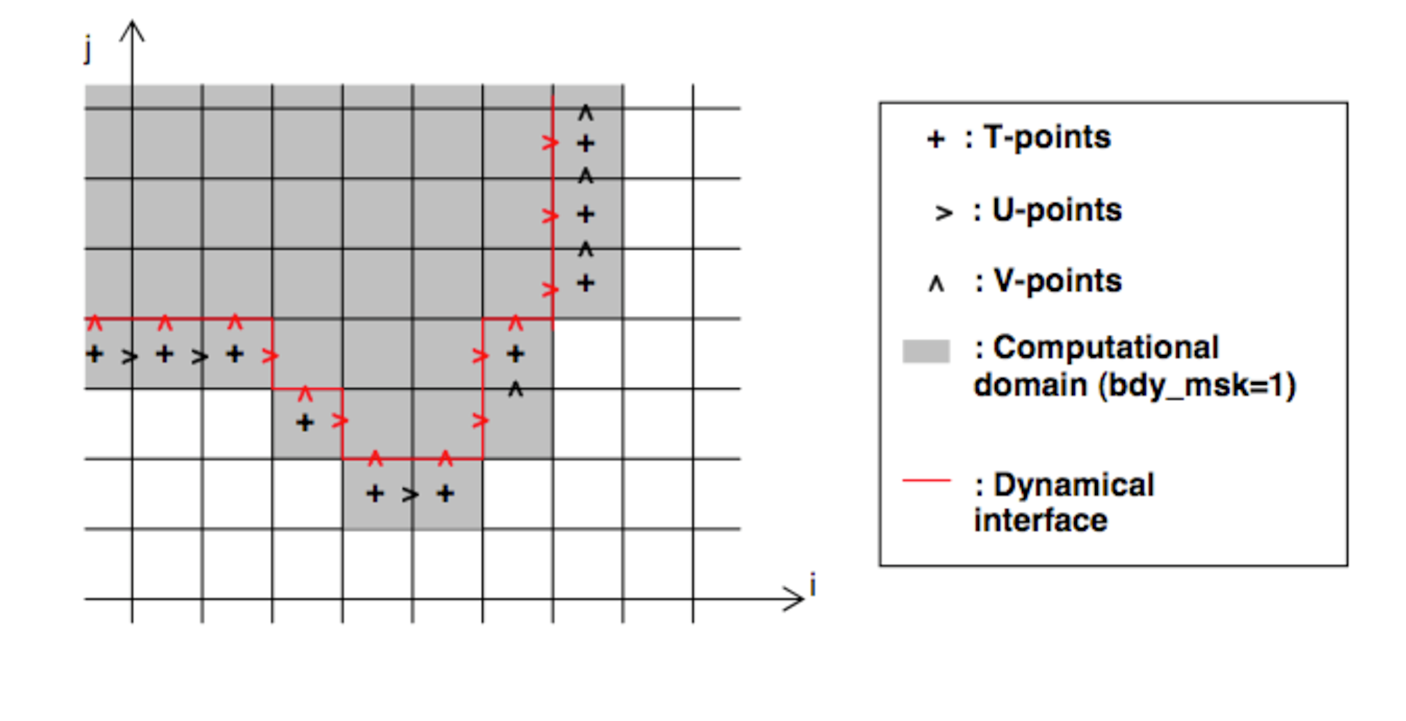
\includegraphics[width=1.0\textwidth]{./TexFiles/Figures/Fig_LBC_bdy_geom.pdf}
\caption {      \label{Fig_LBC_bdy_geom}
Example of geometry of unstructured open boundary}
\end{center}   \end{figure}
%>>>>>>>>>>>>>>>>>>>>>>>>>>>>


\subsection{Defining the regional domain}
\label{domain}

2 options:

read in mask - how is this defined : netcdf file listed in namelist? if not present gui pops up?

generate new mask using gui


\section{Grid Information}
\label{s_coord}
%--------------------------------------------namvert-------------------------------------------------------
\namdisplay{./TexFiles/Namelist/namgrd.nml} 
%--------------------------------------------------------------------------------------------------------------

There is no clean way given a coordinates.nc file and bathymetry.nc file to generate the grid information
from the proposed regional simulation, without replicating a lot of the domzgr.F90  code. At this early stage
in writing BDY tools it was deamed cleaner and safer if this information is required as input. This is easily 
achieved by running the proposed regional simulation for a single timestep with \np{nn\_msh} set to 3 in the 
\NEMO namelist file. This will output 3 files: msh\_hgr.nc, msh\_zgr.nc and mask.nc.
A mask from the source grid is also required (\np{cn\_src\_msk}). It is often the case the data have
be post processed and are missing relavent meta data to determine where the land ocean divide 
is (e.g. the land values in an ice field are set to zero). The tools rely on the masks and do not 
search for missing\_value or \_FillValue properties as these have been found to be unreliable. 
However, scale\_factor and off\_set are still read from the source files if they exist and applied to
the relevant data.

\section{Vertical coordinate}
\label{vert_coord}
%--------------------------------------------namvert-------------------------------------------------------
\namdisplay{./TexFiles/Namelist/namvert.nml} 
%--------------------------------------------------------------------------------------------------------------




\subsection{S-coordinate}
\label{s_coord}
%--------------------------------------------namvert-------------------------------------------------------
\namdisplay{./TexFiles/Namelist/namsco.nml} 
%--------------------------------------------------------------------------------------------------------------


\subsection{unstructured open boundaries options}
\label{bdyopts}




\subsection{Post Extraction}
\label{pe}
%--------------------------------------------namvert-------------------------------------------------------
\namdisplay{./TexFiles/Namelist/namextra.nml} 
%--------------------------------------------------------------------------------------------------------------

weighting gauss nearest linear bicube?
the use of weighting function - auto generate to right length? truncated by fr smoothing red
use of fr / auto? / 
fr in search and fr in smoothing
fr set to small is nearest neighbour (talk in terms of grid res + pictorial e.g.)





%----------------------------------------------

%----------------------------------------------
\subsection{Input boundary data files}
\label{BDY_data}

The data files contain the data arrays
in the order in which the points are defined in the $nbi$ and
$nbj$
arrays. The data arrays are dimensioned on: a time dimension;
$xb$ which is the index of the boundary data point in the
horizontal;
and $yb$ which is a degenerate dimension of 1 to enable the file
to be
read by the standard NEMO I/O routines. The 3D fields also have
a
depth dimension. 

At Version 3.4 there are new restrictions on the order in which
the
boundary points are defined (and therefore restrictions on the
order
of the data in the file). In particular:

\mbox{}

\begin{enumerate}
\item The data points must be in order of increasing $nbr$, ie.
all
  the $nbr=1$ points, then all the $nbr=2$ points etc.
\item All the data for a particular boundary set must be in the
same
order. (Prior to 3.4 it was possible to define barotropic data
in a
different order to the data for tracers and baroclinic
velocities).
\end{enumerate}

\mbox{}

These restrictions mean that data files used with previous
versions of
the model may not work with version 3.4. A fortran utility
{\it bdy\_reorder} exists in the TOOLS directory which will
re-order the
data in old BDY data files. 

%>>>>>>>>>>>>>>>>>>>>>>>>>>>>
\begin{figure}[!t]     \begin{center}
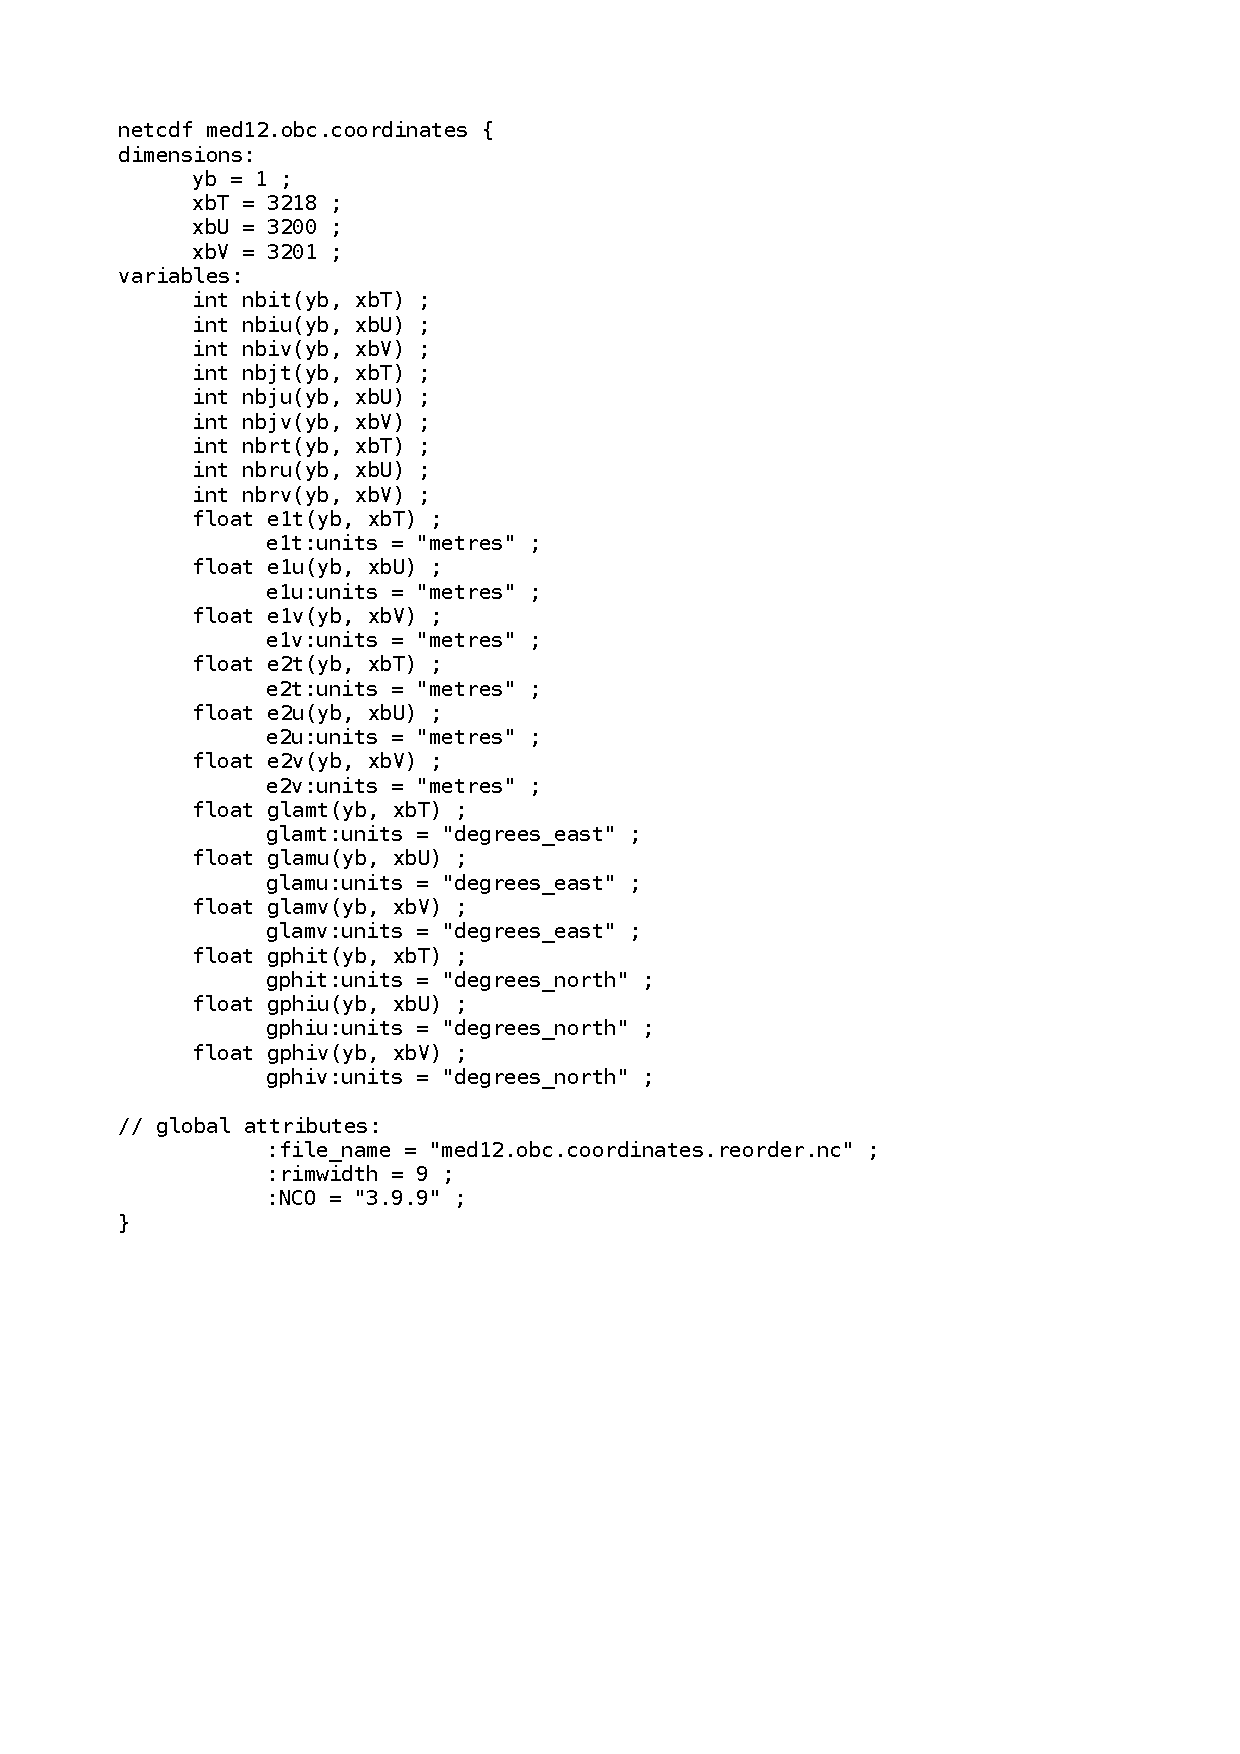
\includegraphics[width=1.0\textwidth]{./TexFiles/Figures/Fig_LBC_nc_header.pdf}
\caption {     \label{Fig_LBC_nc_header} 
Example of the header for a coordinates.bdy.nc file}
\end{center}   \end{figure}
%>>>>>>>>>>>>>>>>>>>>>>>>>>>>

%----------------------------------------------

\subsection{Debugging}
\label{Debug}




%
================================================================
% Chapter � BDY TOOLS Quick Start Guide
%
================================================================
\chapter{Examples}
\label{eq}

$\ $\newline    % force a new ligne


%gm% add here introduction to this chapter

%
\noindent ================================================================
% Boundary Condition at the Coast
%
================================================================

\section{Simple box domain}
\label{box}

\section{AMM12}
\label{amm}



%----------------------------------------------





% bit on code style , harmonisation, f-c and python coding conventions

% ================================================================
% INDEX
% ================================================================

\addcontentsline{toc}{chapter}{Index}
\printindex

% ================================================================
% BIBLIOGRAPHY
% ================================================================

%%\bibliographystyle{plainat}
\bibliographystyle{./TexFiles/ametsoc}		% AMS biblio style (JPO)
\bibliography{./TexFiles/Biblio/Biblio}

% ================================================================
\end{document}
